\documentclass[xcolor=dvipsnames]{beamer}

%\usetheme{Darmstadt}

\usetheme{CambridgeUS}
\usecolortheme{lily}

%\usecolortheme{beaver}

%\setbeamerfont{block title}{size={}}
%\setbeamercolor{title}{bg=blue, fg=white}
%\setbeamercolor{structure}{bg=blue, fg=white}


%\includeonlyframes{current}

\usepackage{times}
\usefonttheme{structurebold}

\usepackage{listings}
\usepackage{pgf}
\usepackage{tikz}
\usepackage{alltt}
\usepackage{verbatim}
\usepackage[normalem]{ulem}
\usetikzlibrary{arrows}
\usetikzlibrary{automata}
\usetikzlibrary{shapes}
\usepackage{amsmath,amssymb, amsxtra}
\usepackage{rotating}
\usepackage[lined,boxed,resetcount]{algorithm2e}
\usepackage{proof}
%For removing the institution name in the footers of the slides
    \defbeamertemplate*{footline}{my infolines theme}
    {
      \leavevmode%
      \hbox{%
      \begin{beamercolorbox}[wd=.333333\paperwidth,ht=2.25ex,dp=1ex,center]{author in head/foot}%
        \usebeamerfont{author in head/foot}\insertshortauthor~~\insertshortinstitute
      \end{beamercolorbox}%
      \begin{beamercolorbox}[wd=.333333\paperwidth,ht=2.25ex,dp=1ex,center]{title in head/foot}%
        \usebeamerfont{title in head/foot}\insertshorttitle
      \end{beamercolorbox}%
      \begin{beamercolorbox}[wd=.333333\paperwidth,ht=2.25ex,dp=1ex,right]{date in head/foot}%
        \usebeamerfont{date in head/foot}\insertshortdate{}\hspace*{2em}
        \insertframenumber{} / \inserttotalframenumber\hspace*{2ex}
      \end{beamercolorbox}}%
      \vskip0pt%
    }

%\setbeamercovered{dynamic}

\title[Static Taint Analysis for C with LLVM]
{Static Taint Analysis for C with LLVM}

\author[]{Xavier Noumbissi}
\institute[ECE 750 (Spring 2013)]{Department of Electrical and Computer Engineering\\ University of Waterloo}
\date{}

\colorlet{redshaded}{red!25!bg}
\colorlet{shaded}{black!25!bg}
\colorlet{shadedshaded}{black!10!bg}
\colorlet{blackshaded}{black!40!bg}

\colorlet{darkred}{red!80!black}
\colorlet{darkblue}{blue!80!black}
\colorlet{darkgreen}{green!80!black}

\newcommand{\rot}[1]{\rotatebox{90}{\mbox{#1}}}
\newcommand{\gray}[1]{\mbox{#1}}
\newtheorem{prop}{Proposition}

\newcounter{myBase}
\newcounter{myCurrent}[myBase]
\setcounter{myBase}{0}
\setcounter{myCurrent}{0}

\newcommand{\inCnt}{\addtocounter{myCurrent}{1}}
\newcommand{\rstCnt}{ \stepcounter{myBase} }

%%% Command for code embedding
\newcommand{\EmbedCode}[3]{
	\lstset{language=#1}
	\lstset{basicstyle=\small,
			linewidth=10cm,
			commentstyle=\textit,
			keywordstyle=,
			stringstyle=\ttfamily,
			showspaces=false,
			numbers=#3,
			stepnumber=1,
			numberfirstline=false,
			numberblanklines=false,
			frame=none,
			showstringspaces=false,
			xleftmargin=0pt
			}
	\lstinputlisting[]{#2} 
}

\newcommand{\EmbedCodeTiny}[3]{
	\lstset{language=#1}
	\lstset{basicstyle=\tiny,
			linewidth=6cm,
			commentstyle=\textit,
			keywordstyle=,
			stringstyle=\ttfamily,
			showspaces=false,
			numbers=#3,
			stepnumber=1,
			numberfirstline=false,
			numberblanklines=false,
			frame=none,
			showstringspaces=false,
			xleftmargin=10pt}
	\lstinputlisting[]{#2} 
}

\newcommand{\EmbedCodeTinyMarg}[4]{
	\lstset{language=#1}
	\lstset{basicstyle=\tiny,
			linewidth=6cm,
			commentstyle=\textit,
			keywordstyle=,
			stringstyle=\ttfamily,
			showspaces=false,
			numbers=#3,
			stepnumber=1,
			numberfirstline=false,
			numberblanklines=false,
			frame=none,
			showstringspaces=false,
			xleftmargin=#4pt}
	\lstinputlisting[]{#2} 
}

\newcommand{\ov}[	1]{\overline{#1}}

%%for source code embedding
\definecolor{listingray}{gray}{0.9}
\definecolor{lbcolor}{rgb}{0.9,0.9,0.9}

\begin{document}

\begin{frame}
  \titlepage
\end{frame}

%\begin{frame} \small
  %\frametitle{Outline}
  %\tableofcontents[subsectionstyle=hide]  
%\end{frame}

%%%%%%%%%%%%%%%%%%%%%%%%%% MOTIVATIONS %%%%%%%%%%%%%%%%%%%%%%%%%
\begin{frame}
  \frametitle{Problem: Prevent Software Vulnerabilities} {\Large	
	\begin{itemize}
	 \item Format String Attacks
	 \vspace{0.5cm}
	 \item SQL Injection
	 \vspace{0.5cm}
	 \item Cross Site Scripting, etc.
	\end{itemize}  
	}
\end{frame}

\begin{frame}
  \frametitle{Solution: Track Used of Non Trusted Program Input} {\Large
   \begin{itemize}
	\item Non trusted program input: \textcolor{red}{Tainted Input}
   	\vspace{0.5cm}	
	\item Source: origin of tainted input
   	\vspace{0.5cm}
	\item Sink: use of tainted input
   	\vspace{0.5cm}
	\item Taint Propagation: tracking tainted input
	\end{itemize}
	}
\end{frame}

\begin{frame}
  \frametitle{Example} 
    {\small
	\begin{center}
	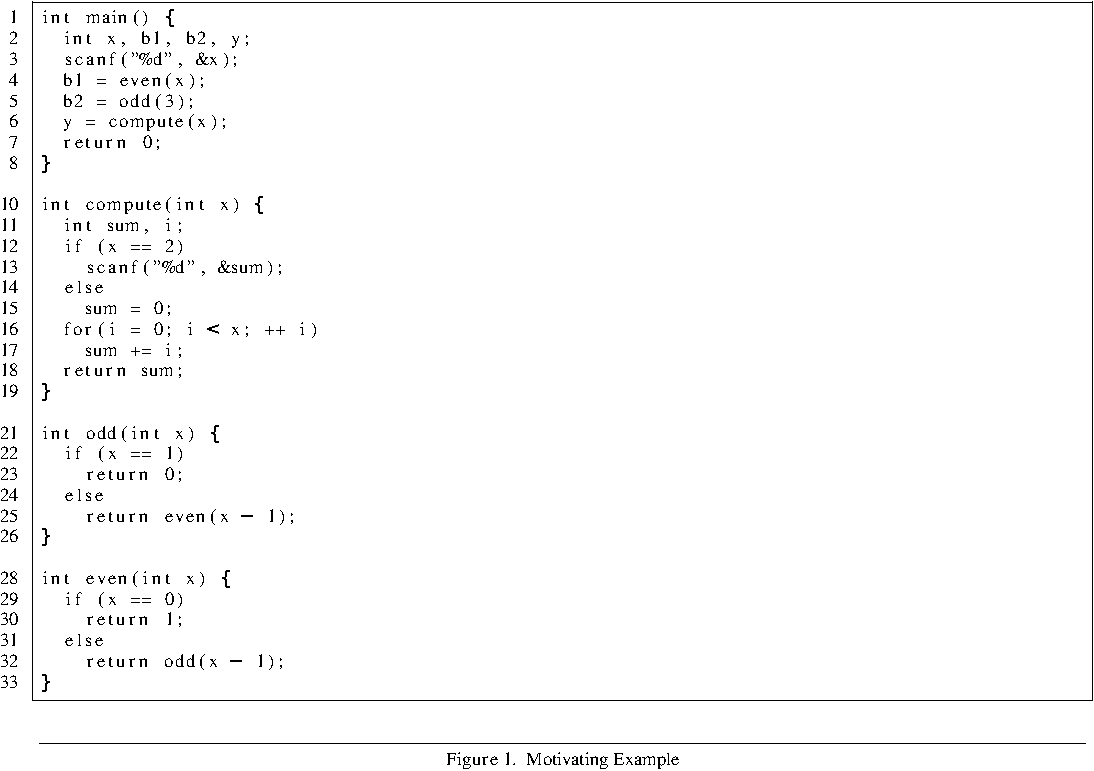
\includegraphics[scale=0.55]{example}
	\end{center}   
	}
\end{frame}

\begin{frame}
  \frametitle{Solution: In This Project} {\Large
   \begin{itemize}
	\item Implicit Taint Propagation: due to \textcolor{blue}{Control Flow}
   	\vspace{0.5cm}	
	\item Explicit Taint Propagation: due to \textcolor{green}{Data Flow}
	\end{itemize}
	}
\end{frame}

\begin{frame}
  \frametitle{Expected Contributions} 
	{\Large
	\begin{itemize}
	\item Algorithm to statically detect use of tainted values in C programs
   	\vspace{0.5cm}
	\item Handling of interprocedural taint propagation
   	\vspace{0.5cm}   	
	\item Implementation of the algorithm in LLVM
	\end{itemize}
	}
\end{frame}

\begin{frame}
  \frametitle{Taint Analysis: Relevant C Program Statements} 
	\Large
\begin{center}
\begin{tabular}{|l|l|}
\hline
Statement Type 				& C Code 			\\ \hline
\hline
\textcolor{blue}{COPY}		& $p = q$				\\	\hline
\textcolor{blue}{LOAD}		& $p = *q$				\\ 	\hline
\textcolor{blue}{STORE}		& $*p = q$				\\ 	\hline
\textcolor{blue}{ADDROF}	& $p = \&a$				\\ 	\hline
\textcolor{blue}{SOURCE}	& $\mathit{call\ gets}  $ \\ 	\hline
\end{tabular}
\end{center}    	
\end{frame}

\begin{frame}
  \frametitle{Taint Analysis: Transfer Functions} 
	{\large
	\begin{itemize}
	\item \textcolor{blue}{COPY}\ [$p = q$]: \textcolor{red}{taint p} iff q is tainted
   	\vspace{0.2cm}	
	\item \textcolor{blue}{LOAD}\ [$p = *q$]: \textcolor{red}{taint p} iff it exists $t_q = *q \wedge t_q$ is tainted
   	\vspace{0.2cm}		
	\item \textcolor{blue}{STORE}\ [$*p = q$]: \textcolor{green}{nothing}
   	\vspace{0.2cm}		
	\item \textcolor{blue}{ADDROF}\	[$p = \&a$]: \textcolor{green}{nothing}
   	\vspace{0.2cm}		
	\item \textcolor{blue}{SOURCE}\	 [$\mathit{call\ gets(p)}$]: \textcolor{red}{taint all} $t_q\ \mathtt{s.t}\ t_q = *p$ 
	\end{itemize}
}
\end{frame}

\begin{frame}
  \frametitle{Interprocedural, Context-Sensitive Analysis} {
   \Large
   \begin{itemize}
	\item Analysis of a callee start with the taint assumptions from the caller
	%\vspace{0.5cm}
	%\item Offline Phase: aggregates results from online phase 
	\end{itemize}
	}
\end{frame}

\begin{frame}
  \frametitle{Taint Information from Source} 
    {\Large
	\begin{itemize}
	\item Developer specify sources and sinks in configuration file
   	\vspace{0.2cm}	
   	\item Analysis do not analyze sources and sinks
   	\vspace{0.2cm}	     	   		   	
   	\item Analysis use annotations for sources: taint propagation
   	\end{itemize}
	}
\end{frame}

\begin{frame}
  \frametitle{Algorithm Analyze: Implements Interprocedural Analysis} 
    {\small
	\begin{center}
	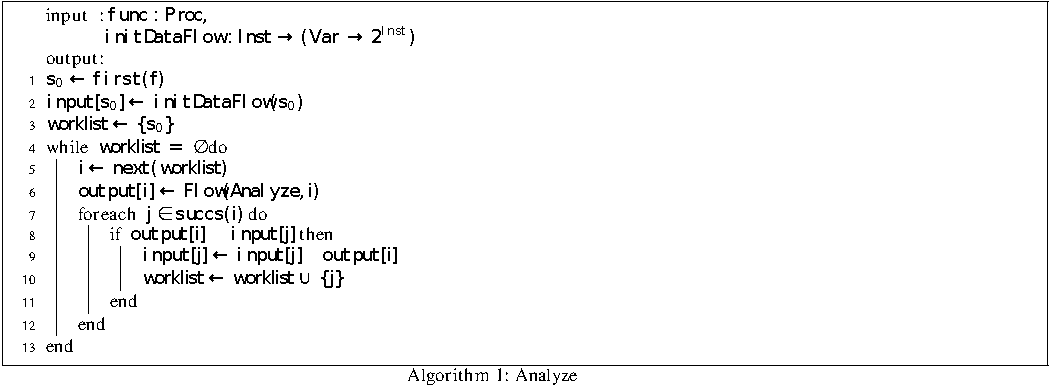
\includegraphics[scale=0.65]{analyze}
	\end{center}   
	}
\end{frame}

\begin{frame}
  \frametitle{Algorithm Flow: Implements Transfer Functions} 
    {\small
	\begin{center}
	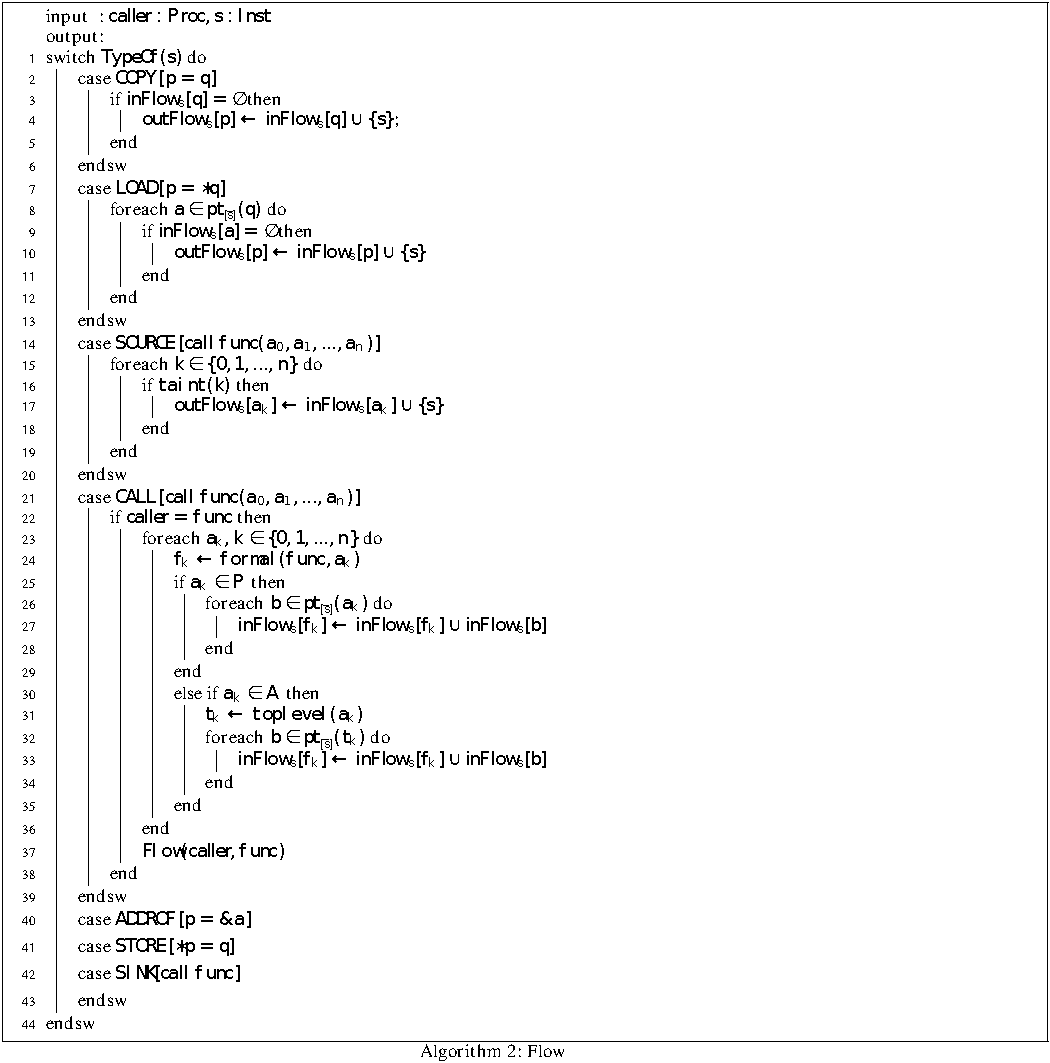
\includegraphics[scale=0.45]{flow}
	\end{center}   
	}
\end{frame}

\begin{frame}
  \frametitle{Implementation} {
   \Large
	\begin{itemize}
	\item LLVM infrastructure is ready
	\vspace{0.5cm}
	\item Need to implement the analysis	
	\end{itemize}   
	}
\end{frame}


\begin{frame}
  \frametitle{Future Work} {
   \Large
	\begin{itemize}
	\item Make analysis modular
	\vspace{0.5cm}	
	\item Better handling of (mutual-) recursive function calls
	\end{itemize}   
	}
\end{frame}

\begin{frame}
  \frametitle{Conclusion} {
   \Large
	\begin{itemize}
	\item Implementation should take less than 1 months
	\vspace{0.5cm}
	\item Need to do evaluation on real world C programs
	\vspace{0.5cm}	
	\item We are optimistic about future results
	\end{itemize}   
	}
\end{frame}

\begin{frame}
  \frametitle{} {\LARGE
\begin{center}
\textbf{Thank You!}
\end{center}
}
\end{frame}

\begin{frame}
  \frametitle{} {\LARGE
\begin{center}
\textbf{Comments \& Questions}
\end{center}
}
\end{frame}

\end{document}